% Detour Steer - สรุป (ภาษาไทย). Build: xelatex (twice), inside algorithm_sim/docs
\documentclass[11pt,a4paper]{article}
\usepackage[top=1.6cm,bottom=1.6cm,left=2cm,right=2cm]{geometry}
\usepackage{amsmath,amssymb}
\usepackage{mathpazo}
\usepackage{fontspec}
\setmainfont{Leelawadee UI}[Scale=0.92, BoldFont={Leelawadee UI Bold}]
\setmonofont{Consolas}[Scale=0.9]
\XeTeXlinebreaklocale "th"
\XeTeXlinebreakskip = 0pt plus 1pt
\linespread{1.12}
\usepackage{booktabs}
\usepackage[linesnumbered,lined]{algorithm2e}
\usepackage{graphicx}
\usepackage{url}
\usepackage[hidelinks]{hyperref}
\RestyleAlgo{boxed}
\SetAlgoNlRelativeSize{-1}
\newcommand{\algcommentfont}[1]{\footnotesize\textnormal{#1}}
\SetCommentSty{algcommentfont}
\SetKwComment{tcp}{/\kern-0.12em/\ }{}
\SetKwProg{Pro}{Procedure :}{}{end}
\SetFuncSty{textit}
\SetKwFunction{FPlan}{PlanLeg}
\setlength{\parindent}{0pt}
\setlength{\parskip}{3pt}
\usepackage{titlesec}
\titlespacing*{\section}{0pt}{2.2ex}{0.8ex}
\pagestyle{empty}

\begin{document}
\begin{flushright}{\small\bfseries Phuthiphong Wongchantib 660610840}\end{flushright}
\vspace{-3mm}
\begin{center}
{\Large\bfseries Detour Steer --- สรุป}\\[1mm]
อัลกอริทึมตัดสินใจของหุ่นที่เลี้ยวได้ทางเดียว: วิ่งไปก่อน เลี้ยวให้น้อยลง แล้วค่อยเข้าเป้า
\end{center}

\section*{1. ปัญหา}
หุ่น \texttt{mor\_luam} มี\textbf{มอเตอร์ตัวเดียว} หมุนทางหนึ่งเป็นการ\emph{เลี้ยว}ล้อ (ได้แค่ทวนเข็มนาฬิกา)
หมุนอีกทางเป็นการ\emph{วิ่ง}ไปข้างหน้า หุ่นจึงต้อง\textbf{หยุดก่อนเลี้ยว} และเลี้ยวขณะวิ่งไม่ได้
วิธีเดิมคือเลี้ยวตรงไปหาเป้าก่อนแล้วค่อยวิ่ง ถ้าเป้าอยู่ทาง\textbf{ขวา}นิดเดียว ($\varphi$ ใกล้ $360^\circ$)
ล้อต้องหมุนเกือบรอบ

\section*{2. แนวคิด}
เส้นตรงสองช่วงที่ทิศต่างกันเกิน $180^\circ$ ไปถึงได้ทุกทิศ แทนที่จะเลี้ยว $\varphi$ หุ่นเลือกได้ว่าจะ:
\begin{enumerate}\setlength\itemsep{0pt}
\item วิ่งตรงไปก่อน $a$ เมตร (ไม่เลี้ยว)
\item เลี้ยวแค่ $\beta^\ast$ \;($180^\circ < \beta^\ast < \varphi$)
\item วิ่งอีก $b$ เมตรถึงเป้า
\end{enumerate}
มุมที่ดีที่สุดมีสูตรปิด (ตัวเลข $k$ ตัวเดียวตัดสินทุกอย่าง):
\[
k = \frac{d\,\omega}{v}\,\lvert\sin\varphi\rvert,\qquad
\beta^\ast = 360^\circ - \arccos(k-1),\qquad
a = \frac{d\,\sin(\beta^\ast-\varphi)}{\sin\beta^\ast},\qquad
b = \frac{d\,\sin\varphi}{\sin\beta^\ast}
\]
$d$ = ระยะถึงเป้า, $\omega$ = ความเร็วเลี้ยว, $v$ = ความเร็ววิ่ง,
$t_s$ = เวลารอล้อนิ่ง, $t_b$ = เวลาหยุดระหว่างสองช่วง

\section*{3. อัลกอริทึมตัดสินใจ}
{\small
\begin{algorithm}[H]
\Pro(\tcp*[f]{$\varphi$: มุมทวนเข็มไปหาเป้า, $d$: ระยะ}){\FPlan{$\varphi$, $d$}}{
  $T_D \leftarrow \varphi/\omega + t_s + d/v$\tcp*[r]{วิธีเดิม: เลี้ยว $\varphi$ แล้ววิ่ง $d$}
  \lIf(\tcp*[f]{T1: เลี้ยวตรงไปดีที่สุด}){$\varphi \le 180^\circ$}{\KwRet{DIRECT}}
  $k \leftarrow (d\,\omega/v)\,\lvert\sin\varphi\rvert$\;
  \lIf(\tcp*[f]{T3: อ้อมแบบไหนก็ไม่เร็วกว่า}){$k \ge 2$}{\KwRet{DIRECT}}
  $\beta^\ast \leftarrow 360^\circ - \arccos(k-1)$;\quad คำนวณ $a$, $b$\;
  $T_R \leftarrow a/v + t_b + \beta^\ast/\omega + t_s + b/v$\;
  \lIf(\tcp*[f]{อ้อมเฉพาะเมื่อเร็วกว่าจริง}){$\beta^\ast < \varphi$ \textbf{and} $T_R < T_D$}{\KwRet{DETOUR($a$, $\beta^\ast$, $b$)}}
  \KwRet{DIRECT}\;
}
\end{algorithm}
}
หุ่นเรียกฟังก์ชันนี้\textbf{ใหม่หลังขยับทุกครั้ง} (วงปิด) โดยใช้มุมล้อจริง (AS5600) และทิศตัวหุ่น (IMU)
ตอนเลี้ยว หุ่นตั้งใจหยุด\emph{ก่อน}ถึงมุมประมาณ $2^\circ$ เพราะขาดแค่เลี้ยวเพิ่มนิดเดียว แต่ถ้าเกินต้องหมุนเกือบรอบ
ตอนวิ่ง หุ่นหยุดก่อนถึงแล้วเล็งใหม่ด้วยการเลี้ยวนิดเดียว ($\approx 18^\circ$)

\section*{4. ทำไมถูกต้องและเร็ว}
\begin{itemize}\setlength\itemsep{0pt}
\item \textbf{T1} ถ้า $\varphi \le 180^\circ$ เลี้ยวตรงไปหาเป้าดีที่สุด
\item \textbf{T2} ถ้า $\varphi > 180^\circ$ เส้นทางที่ดีที่สุดมีไม่เกิน 2 ช่วง
\item \textbf{T3} เวลามีจุดต่ำสุดจุดเดียว ที่ $\cos\beta^\ast = k-1$
\item \textbf{T4} วางแผนใหม่หลังวิ่งช่วงแรก แผนยังเหมือนเดิม วงปิดจึงไม่แกว่ง
\item \textbf{O(1)} ต่อการตัดสินใจหนึ่งครั้ง: 0.54\,$\mu$s ใน Python เร็วกว่าการค้นหา 3600 จุด $944\times$
      T1--T4 ตรวจแบบ brute force ใน \texttt{detour\_steer.py} ผ่านทั้งหมด
\end{itemize}

\section*{5. ผลลัพธ์}
\textbf{ซิม} (เป้าสุ่ม 5000 จุด): Detour Steer ไม่ช้ากว่าวิธีเดิมเลย
ประหยัด 0.4\,\% เมื่อล้อหยุดตรงพอดี, 2.3--6.9\,\% เมื่อล้อหยุดคลาดแบบสุ่ม
และ 12.8--18.3\,\% เมื่อล้อมักหยุดเกินมุม

\textbf{บนหุ่นจริง} (เป้าห่าง 0.30\,m ที่ $\varphi = 354^\circ$, $v = 0.03$\,m/s, $\omega = 35^\circ$/s, 3 รอบ):
\begin{center}
\begin{tabular}{lrrr}
\toprule
รอบ & วิธีเดิม (s) & Detour Steer (s) & ประหยัด (s)\\
\midrule
1 & 24.17 & 20.83 & 3.34\\
2 & 22.94 & 20.77 & 2.17\\
3 & 23.36 & 22.33 & 1.03\\
\midrule
เฉลี่ย & 23.49 & 21.31 & 2.18 (9.3\,\%)\\
\bottomrule
\end{tabular}
\end{center}
Detour Steer ชนะทั้ง 3 รอบ เลี้ยวน้อยลง 3.8\,s และวิ่งนานขึ้น 1.2\,s
ทั้ง 6 รอบหยุดห่างเป้าไม่เกิน 2.5\,mm

\begin{center}
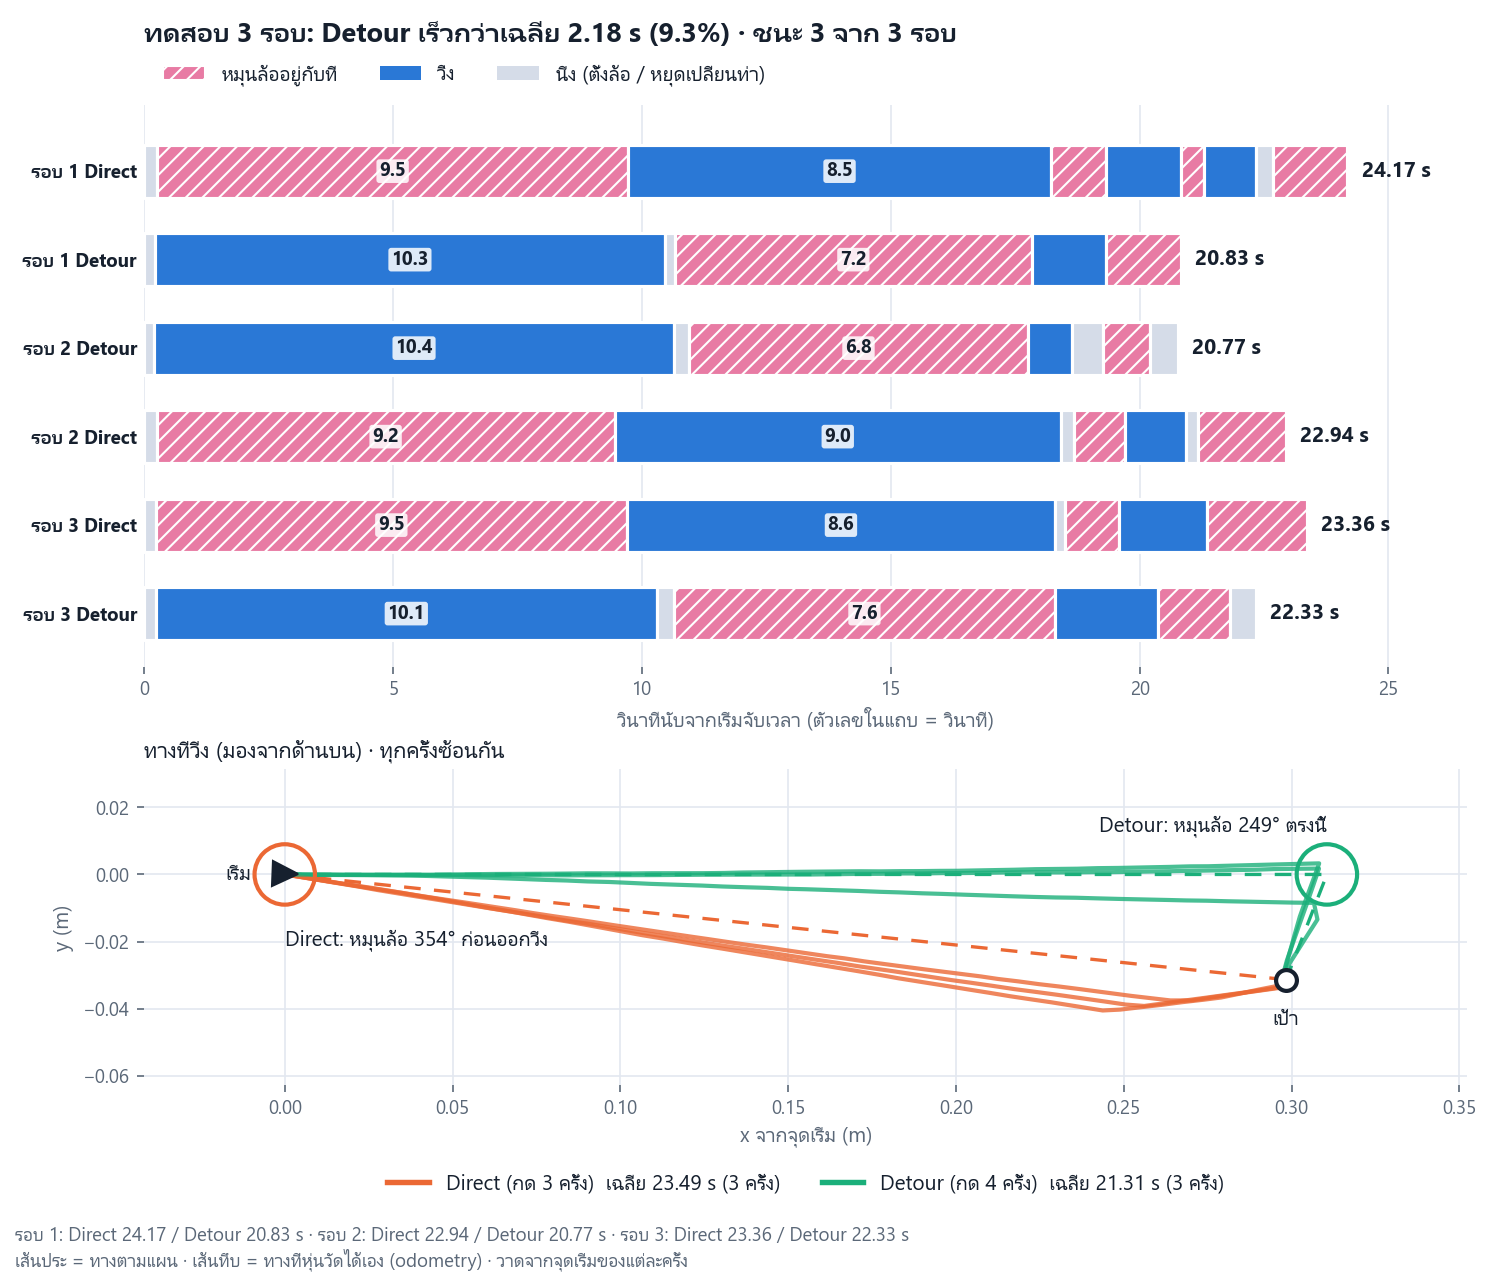
\includegraphics[width=0.74\linewidth]{robot_3rounds.png}\\[-1mm]
{\small รูปที่ 1 ผล 3 รอบจากข้อมูลที่หุ่นบันทึกเอง (บน: เวลาแต่ละช่วง, ล่าง: เส้นทางที่วัดได้)}
\end{center}

\section*{6. สรุป}
กฎสูตรปิดข้อเดียวตัดสินว่าจะ ``เลี้ยวตรงไป'' หรือ ``วิ่งไปก่อน เลี้ยวให้น้อยลง แล้วค่อยเข้าเป้า''
ใช้เวลา $O(1)$ ต่อการตัดสินใจ ไม่ช้ากว่าวิธีเดิมในซิม และเร็วขึ้น 9.3\,\% บนหุ่นจริง
ยังไม่พบงานอื่นที่ให้สูตรปิดของการอ้อมแบบนี้ สำหรับหุ่นที่ต้องหยุดก่อนเลี้ยวและเลี้ยวได้ทางเดียว
(``ไม่พบ'' ไม่ได้พิสูจน์ว่าไม่มีใครเคยทำ)

\clearpage
\section*{โค้ด Git และวิดีโอ}
โค้ดทั้งหมด (ตัววางแผน Python, ซิม, เฟิร์มแวร์บนหุ่น) และรายงานฉบับเต็ม:
\begin{center}\large\url{https://github.com/Mannaja78520/mor_luam}\end{center}
\begin{itemize}\setlength\itemsep{0pt}
\item ตัววางแผนและซิม: \texttt{algorithm\_sim/} (รันได้โดยไม่ต้องใช้ Docker: \texttt{pip install matplotlib})
\item บนหุ่นจริง: \texttt{firmware/src/algorithm/DetourSteer.cpp}
\item รายงานฉบับเต็ม: \texttt{algorithm\_sim/docs/660610840\_DetourSteer.pdf} (ไทย), \texttt{report.pdf} (อังกฤษ)
\item วิธีติดตั้ง: \texttt{algorithm\_sim/README.md}, \texttt{docs/INSTALL\_TH.md} (แนะนำติดตั้งแบบ Docker)
\end{itemize}

\textbf{วิดีโอการทำงานของหุ่น:}
\begin{center}\url{https://drive.google.com/drive/folders/11qOM6UoeH2c4nEuM0a0JO6eXTnr0eDud}\end{center}
{\small คลิปนี้เป็นการทำงานของหุ่นแบบ synchronize
ไม่มีคลิปของการเปรียบเทียบ Detour Steer กับวิธีเดิม (Direct)
ผลการเปรียบเทียบดูได้จากข้อมูลที่หุ่นบันทึกเองในรูปที่ 1 และตารางผลบนหุ่นจริง}
\end{document}
